\documentclass[12pt, varwidth=true, border=10pt, convert={size=640x}]{standalone}

\usepackage{amsmath,amssymb,bm}
\usepackage[table]{xcolor}
\usepackage{tikz}
\usetikzlibrary{positioning,calc,intersections,arrows,decorations.pathreplacing}
\usepackage{pgfplots}
%\pgfplotsset{compat=1.14}
\usepackage{fullpage}

  \usepackage[T1]{fontenc}
  \usepackage[utf8]{inputenc}
%  \usepackage{stix}
  \usepackage[default]{opensans}
  \renewcommand{\ttdefault}{lmtt}

\usepackage{blkarray}

\begin{document}
%\thispagestyle{empty}

\begin{center}

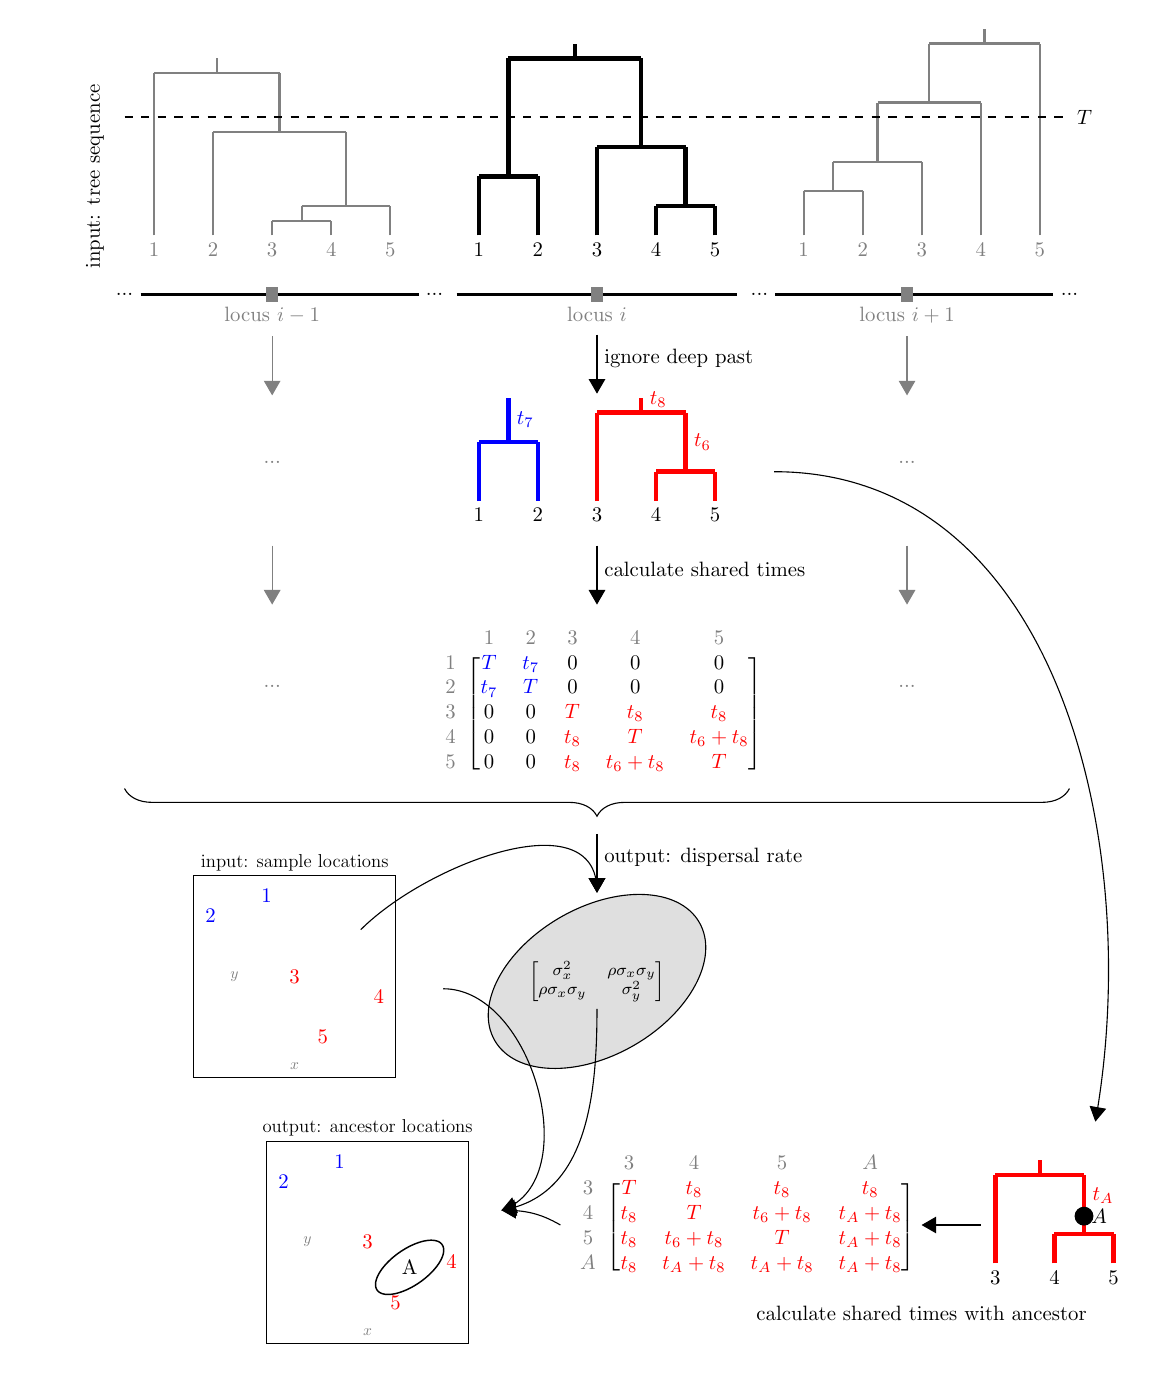
\begin{tikzpicture}[>=triangle 60, scale=0.75, every node/.style={scale=0.75}] %if figure too big, adjust both scales equally

%%%%%%%%%%
%tree sequence
%%%%%%%%%%

%%%%%%%%%%%%%%%
%genome
  \node[] (gleft) at (-8,-1) {...};
  \node[] (gright) at (-2.75,-1) {...};
  \draw[thick] (gleft) -- (gright);
  \node[] (gleft) at (-2.5,-1) {};
  \node[] (gright) at (2.5,-1) {};
  \draw[thick] (gleft) -- (gright);
  \node[] (gleft) at (2.75,-1) {...};
  \node[] (gright) at (8,-1) {...};
  \draw[thick] (gleft) -- (gright);
  \coordinate (gleft) at (-8,-1);
  \coordinate (gright) at (8,-1);
  
%%%%%%%%%%%%%%
%focal tree
  
  %location on genome
  \coordinate (tree) at (0,0);
  \draw[line width=2mm, gray] (-0.1,-1) -- (0.1,-1) node[midway, below] (locus) {locus $i$};
  
  % sample nodes
  \foreach \n in {1,...,5}{
    \coordinate (n\n) at (\n - 3, 0); % define coordinate
    \node[below = 0cm of n\n] {\n}; %node label
  }
  % ancestor node 1
  \foreach \t in {0.5}{
    \foreach \n in {4,5}{
      \draw[ultra thick] (n\n) -- (n\n |- 0,\t);
    }
  \draw[ultra thick] (n4 |- 0,\t) -- (n5 |- 0,\t) coordinate[midway] (n6);
  }    
  % ancestor node 2
  \foreach \t in {1}{ %coalescent time
    \foreach \n in {1,2}{ %nodes that coalesce
      \draw[ultra thick] (n\n) -- (n\n |- 0,\t);
    }
  \draw[ultra thick] (n1 |- 0,\t) -- (n2 |- 0,\t) coordinate[midway] (n7);
  }
  % ancestor node 3
  \foreach \t in {1.5}{
    \foreach \n in {3,6}{
      \draw[ultra thick] (n\n) -- (n\n |- 0,\t);
    }
  \draw[ultra thick] (n3 |- 0,\t) -- (n6 |- 0,\t) coordinate[midway] (n8);
  }  
  % ancestor node 4
  \foreach \t in {3}{
    \foreach \n in {7,8}{
      \draw[ultra thick] (n\n) -- ( n\n |- 0,\t );
    }
  \draw[ultra thick] ( n7 |- 0,\t ) -- ( n8 |- 0,\t ) coordinate[midway] (n9);
  }
  % mrca stem
  \draw[ultra thick] (n9) -- (n9 |- 0,3.25);      
 
 %%%%%%%%%%%%%%
 %left tree
  
  %location on genome
  \coordinate (tree) at (0,0);
  \draw[line width=2mm, gray] (-5.6, -1) -- (-5.4, -1) node[midway, below] (llocus) {locus $i-1$};
  
  % sample nodes
  \foreach \n in {1,...,5}{
    \coordinate (n\n) at (-6.5 + \n - 2, 0); % define coordinate
    \node[below = 0cm of n\n, gray] {\n}; %node label
  }
  % ancestor node 1
  \foreach \t in {0.25}{
    \foreach \n in {3,4}{
      \draw[thick, gray] (n\n) -- (n\n |- 0,\t);
    }
  \draw[ thick, gray] (n3 |- 0,\t) -- (n4 |- 0,\t) coordinate[midway] (n6);
  }    
  % ancestor node 2
  \foreach \t in {0.5}{ %coalescent time
    \foreach \n in {6,5}{ %nodes that coalesce
      \draw[ thick, gray] (n\n) -- (n\n |- 0,\t);
    }
  \draw[ thick, gray] (n6 |- 0,\t) -- (n5 |- 0,\t) coordinate[midway] (n7);
  }
  % ancestor node 3
  \foreach \t in {1.75}{
    \foreach \n in {2,7}{
      \draw[ thick, gray] (n\n) -- (n\n |- 0,\t);
    }
  \draw[ thick, gray] (n2 |- 0,\t) -- (n7 |- 0,\t) coordinate[midway] (n8);
  }  
  % ancestor node 4
  \foreach \t in {2.75}{
    \foreach \n in {1,8}{
      \draw[ thick, gray] (n\n) -- ( n\n |- 0,\t );
    }
  \draw[thick, gray] ( n1 |- 0,\t ) -- ( n8 |- 0,\t ) coordinate[midway] (n9);
  }
  % mrca stem
  \draw[thick, gray] (n9) -- (n9 |- 0,3); 
  
%%%%%%%%%%%%%%
 %right tree
  
  %location on genome
  \coordinate (tree) at (0,0);
  \draw[line width=2mm, gray] (5.15,-1) -- (5.35,-1) node[midway, below] (rlocus){locus $i+1$};
%  
  % sample nodes
  \foreach \n in {1,...,5}{
    \coordinate (n\n) at (5.5 + \n - 3, 0); % define coordinate
    \node[below = 0cm of n\n, gray] {\n}; %node label
  }
  % ancestor node 1
  \foreach \t in {0.75}{
    \foreach \n in {1,2}{
      \draw[ thick, gray] (n\n) -- (n\n |- 0,\t);
    }
  \draw[ thick, gray] (n1 |- 0,\t) -- (n2 |- 0,\t) coordinate[midway] (n6);
  }    
  % ancestor node 2
  \foreach \t in {1.25}{ %coalescent time
    \foreach \n in {6,3}{ %nodes that coalesce
      \draw[ thick, gray] (n\n) -- (n\n |- 0,\t);
    }
  \draw[ thick, gray] (n6 |- 0,\t) -- (n3 |- 0,\t) coordinate[midway] (n7);
  }
  % ancestor node 3
  \foreach \t in {2.25}{
    \foreach \n in {7,4}{
      \draw[ thick, gray] (n\n) -- (n\n |- 0,\t);
    }
  \draw[ thick, gray] (n7 |- 0,\t) -- (n4 |- 0,\t) coordinate[midway] (n8);
  }  
  % ancestor node 4
  \foreach \t in {3.25}{
    \foreach \n in {8,5}{
      \draw[ thick, gray] (n\n) -- ( n\n |- 0,\t );
    }
  \draw[thick, gray] ( n8 |- 0,\t ) -- ( n5 |- 0,\t ) coordinate[midway] (n9);
  }
  % mrca stem
  \draw[thick, gray] (n9) -- (n9 |- 0,3.5); 
  
%%%%%%%%%%%%%%%%%
%time cut off
\draw[thick, dashed] (-8,2) -- (8,2) node[right] {$T$};
%label
\node[rotate=90] at (-8.5,1) {input: tree sequence};

%%%%%%%%%%%%
% down arrows
\draw[->] (locus.south) -- ($(locus.south) + (0,-1)$) node[midway, right, yshift=0.1cm] {ignore deep past};
\draw[->, gray] (llocus.south) -- ($(llocus.south) + (0,-1)$) node[below, yshift=-1cm] {...};
\draw[->, gray] (rlocus.south) -- ($(rlocus.south) + (0,-1)$) node[below, yshift=-1cm] {...};

%%%%%%%%%%%%%
%subtrees
%%%%%%%%%%%

  % sample nodes
  \foreach \n in {1,...,5}{
    \coordinate (n\n) at (\n - 3, -4.5); % define coordinate
    \node[below = 0cm of n\n] {\n}; %node label
  }
  % ancestor node 1
  \foreach \t in {-4}{
    \foreach \n in {4,5}{
      \draw[ultra thick, red] (n\n) -- (n\n |- 0,\t);
    }
  \draw[ultra thick, red] (n4 |- 0,\t) -- (n5 |- 0,\t) coordinate[midway] (n6);
  }
  % ancestor node 2
  \foreach \t in {-3.5}{ %coalescent time
%    \foreach \n in {1,2}{ %nodes that coalesce
%      \draw[ultra thick] (n\n) -- (n\n |- 0,\t);
%    }
  %\draw[ultra thick, blue] (n1) -- (n1 |- 0,\t)  node[midway, right] {$t_1$}; 
  \draw[ultra thick, blue] (n1) -- (n1 |- 0,\t); 
  \draw[ultra thick, blue] (n2) -- (n2 |- 0,\t); 
  \draw[ultra thick, blue] (n1 |- 0,\t) -- (n2 |- 0,\t) coordinate[midway] (n7);
  }
  % ancestor node 3
  \foreach \t in {-3}{
    %\foreach \n in {3,6}{
    %  \draw[ultra thick, red] (n\n) -- (n\n |- 0,\t) node[midway, right] {$t_\n$};
      %\draw[ultra thick, red] (n\n) -- (n\n |- 0,\t);
    %}
  \draw[ultra thick, red] (n3) -- (n3 |- 0,\t);
  \draw[ultra thick, red] (n6) -- (n6 |- 0,\t) node[midway, right] {$t_6$};
  \draw[ultra thick, red] (n3 |- 0,\t) -- (n6 |- 0,\t) coordinate[midway] (n8);
  }  
  % blue mrca stem
  \draw[ultra thick, blue] (n7) -- (n7 |- 0,-2.75) node[midway, right] {$t_7$}; 
  % red mrca stem
  \draw[ultra thick, red] (n8) -- (n8 |- 0,-2.75) node[midway, right, yshift=0.1cm] {$t_8$}; 
  
%  \node[gray] at (1,-6) {subtree $j$};  

% down arrows
\draw[->] ($(n3.south) + (0,-0.75)$) -- ($(n3.south) + (0,-1.75)$) node[midway, right, yshift=0.1cm] {calculate shared times};
\draw[->, gray] ($(n3.south) + (-5.5,-0.75)$) -- ($(n3.south) + (-5.5,-1.75)$) node[below, yshift=-1.25cm] {...};
\draw[->, gray] ($(n3.south) + (5.25,-0.75)$) -- ($(n3.south) + (5.25,-1.75)$) node[below, yshift=-1.25cm] {...};

%%%%%%%%%%%%
%shared times
%%%%%%%%%%%

  \node[anchor = north] (matrix) at ($(n3.south) + (0,-2)$) {
   $\begin{blockarray}{cccccc}
      & \color{gray}{1} & \color{gray}{2} & \color{gray}{3} & \color{gray}{4} & \color{gray}{5} \\
      \begin{block}{c[ccccc]}
   %$\begin{pmatrix} 
        \color{gray}{1} & \color{blue}{T} & \color{blue}{t_7} & \color{black}{0} & \color{black}{0} & \color{black}{0} \\
        \color{gray}{2} & \color{blue}{t_7} & \color{blue}{T} & \color{black}{0}& \color{black}{0} & \color{black}{0} \\
        \color{gray}{3} & \color{black}{0} & \color{black}{0} & \color{red}{T} & \color{red}{t_8} & \color{red}{t_8} \\ 
        \color{gray}{4} & \color{black}{0} & \color{black}{0} & \color{red}{t_8} & \color{red}{T} & \color{red}{t_6 + t_8} \\ 
        \color{gray}{5} & \color{black}{0} & \color{black}{0} & \color{red}{t_8} & \color{red}{t_6 + t_8} & \color{red}{T} \\
  %\end{pmatrix}$
      \end{block}
   \end{blockarray}$
  };

% down arrows
\draw[decoration={brace,raise=5pt,amplitude=10pt,mirror},decorate] ($(matrix.south) + (gleft) + (0,1.5)$) -- ($(matrix.south) + (gright) + (0,1.5)$);
\coordinate(A) at ($(matrix.south) + (0, -1.5)$);
\draw[->] ($(matrix.south) + (0, -0.5)$) -- (A) node[midway, right, yshift=0.1cm] {output: dispersal rate};

%%%%%%%%%%%%%%
%dispersal rate
%%%%%%%%%%%%%%

\node[anchor=north] at ($(matrix.south) + (gleft) + (0, -3.5)$) (locations) {
  \begin{axis}[
      title=input: sample locations,
      title style={at={(axis description cs:0.5,0.95)}, font=\large},
      cycle list name=black white,
      height=5cm,
      width=5cm,
      xlabel=$x$,
      ylabel=$y$,
      samples=5,
      domain=0:1,
      ymin = 0,
      ymax = 1,
      ticks=none,
      x label style={at={(axis description cs:0.5,0.1)}, anchor=north, color=gray},
      y label style={at={(axis description cs:0.25,0.5)},rotate=-90,anchor=east, color=gray}
  ]
%  \addplot+[only marks]  {rand}; %plot some random locations
    \addplot[only marks, mark=text, text mark = {1}, blue] table { 
      0.4 0.9
    };
    \addplot[only marks, mark=text, text mark = {2}, blue] table { 
      0.3 0.8
    };
    \addplot[only marks, mark=text, text mark = {3}, red] table { 
      0.45 0.5
    };
    \addplot[only marks, mark=text, text mark = {4}, red] table { 
      0.6 0.4
    };    
    \addplot[only marks, mark=text, text mark = {5}, red] table { 
      0.5 0.2
    };    
  \end{axis}
};

\draw[->] ($(locations) + (4cm, 2.5cm)$) to [out=45, in=90] (A);

\coordinate(A) at ($(matrix.south) + (0, -3)$);
\draw[fill=lightgray!50!white, rotate around={30:(A)}] (A) ellipse (2cm and 1.25cm);
  \node[] (sigma) at (A) {
  \footnotesize
%   $\widehat{\mathbf{\Sigma}}$
    $\begin{bmatrix} 
      \sigma_x^2 & \rho\sigma_x\sigma_y \\
      \rho\sigma_x\sigma_y & \sigma_y^2
    \end{bmatrix}$
  };

%%%%%%%%%%%%
% locate ancestors
%%%%%%%%%%%%%

% ancestor plot
\node[anchor=north] at ($(matrix.south) + (-7, -9)$) (ancloc) {
  \begin{axis}[
      cycle list name=black white,
      title=output: ancestor locations,
      title style={at={(axis description cs:0.5,0.95)}, font=\large},
      height=5cm,
      width=5cm,
      xlabel=$x$,
      ylabel=$y$,
      samples=5,
      domain=0:1,
      ymin = 0,
      ymax = 1,
      ticks=none,
      x label style={at={(axis description cs:0.5,0.1)}, anchor=north, color=gray},
      y label style={at={(axis description cs:0.25,0.5)},rotate=-90, anchor=east, color=gray}
  ]
%  \addplot+[only marks]  {rand}; %plot some random locations
    \addplot[only marks, mark=text, text mark = {1}, blue] table { 
      0.4 0.9
    };
    \addplot[only marks, mark=text, text mark = {2}, blue] table { 
      0.3 0.8
    };
    \addplot[only marks, mark=text, text mark = {3}, red] table { 
      0.45 0.5
    };
    \addplot[only marks, mark=text, text mark = {4}, red] table { 
      0.6 0.4
    };    
    \addplot[only marks, mark=text, text mark = {5}, red] table { 
      0.5 0.2
    };    
    \addplot[mark=text, text mark = {A}, black] table { 
      0.525 0.375
    };
%    \addplot[domain=0:360,data cs=polar, samples=200, line width=0.7pt, red] (x,{1/(sqrt(1 - 2*cos(x)*cos(x)))});
\addplot [domain=-pi:pi, samples=200, black, line width=0.7pt, rotate around={35:(axis cs:0.525,0.375)}] ({0.525 + sqrt(0.005)*sin(deg(x))}, {0.375 + sqrt(0.008)*cos(deg(x))});
  \end{axis}
};

% shared times
  \node[anchor = west] (vector) at ($(ancloc.east) + (4.5,2)$) {
  % $\left(\begin{array}{>{\columncolor{red!20}}cccc}
  %      \rowcolor{red!20}
  %      \color{red}{t_A} & \color{red}{0} & \color{red}{t_A} & \color{red}{t_A} \\ 
  %      \color{red}{0} & \color{red}{t_3} & \color{red}{0} & \color{red}{0} \\ 
  %      \color{red}{t_A} & \color{red}{0} & \color{red}{t_3} & \color{red}{t_6} \\ 
  %      \color{red}{t_A} & \color{red}{0} & \color{red}{t_6} & \color{red}{t_3} 
  %\end{array}\right)$
    $\begin{blockarray}{ccccc}
      & \color{gray}{3} & \color{gray}{4} & \color{gray}{5} & \color{gray}{A} \\
      \begin{block}{c[cccc]}
        \color{gray}{3} & \color{red}{T} & \color{red}{t_8} & \color{red}{t_8} & \color{red}{t_8} \\
        \color{gray}{4} & \color{red}{t_8} & \color{red}{T} & \color{red}{t_6 + t_8} & \color{red}{t_A + t_8} \\
        \color{gray}{5} & \color{red}{t_8} & \color{red}{t_6 + t_8} & \color{red}{T} & \color{red}{t_A + t_8} \\
        \color{gray}{A} & \color{red}{t_8} & \color{red}{t_A + t_8} & \color{red}{t_A + t_8} & \color{red}{t_A + t_8} \\
      \end{block}
    \end{blockarray}$
  };

% red tree
\begin{scope}[shift={($(vector.east) + (1.25,3.85)$)}]

  % sample nodes
  \foreach \n in {3,...,5}{
    \coordinate (n\n) at (\n - 3, -4.5); % define coordinate
    \node[below = 0cm of n\n] {\n}; %node label
  }
  % ancestor node 1
  \foreach \t in {-4}{
    \foreach \n in {4,5}{
      \draw[ultra thick, red] (n\n) -- (n\n |- 0,\t);
    }
  \draw[ultra thick, red] (n4 |- 0,\t) -- (n5 |- 0,\t) coordinate[midway] (n6);
  }    
  % ancestor node 3
  \foreach \t in {-3}{
    \foreach \n in {3,6}{
      \draw[ultra thick, red] (n\n) -- (n\n |- 0,\t);
    }
  \draw[ultra thick, red] (n3 |- 0,\t) -- (n6 |- 0,\t) coordinate[midway] (n8);
  }
  % red mrca stem
  \draw[ultra thick, red] (n8) -- (n8 |- 0,-2.75); 
  % focal ancestor
  \draw[ultra thick, red] (n6 |- 0,-3.7) -- (n6 |- 0,-3) node[midway, right, red] {$t_A$};  
  \draw[fill=black] (n6 |- 0,-3.7) circle (0.15cm) node[right] {$A$};

\end{scope}

%arrows
\draw[->] (3,-4) to [out=0, in=80, looseness=1] ($(vector) + (6,1.75)$);
\draw[->] ($(vector.east) + (1,0)$) -- (vector.east) node[midway, below, xshift=-0.5cm, yshift=-1.25cm] {calculate shared times with ancestor};

% arrows to output
\coordinate(A) at ($(ancloc.east) + (3.5,2.25)$);
\draw[->] ($(locations.east) + (3.75, 1.5)$) to [out=0, in=20] (A);
\draw[->] (vector.west) to [out=150, in=0] (A);
%\draw[->] ($(sigma.south)+(0,0)$) to [out=270, in=10] node[midway, right, xshift=-3cm, yshift=0.5cm, rectangle, fill=white, opacity=0.75, text opacity=1] {output: ancestor locations} (A) ;
\draw[->] ($(sigma.south)+(0,0)$) to [out=270, in=10] (A) ;
%\node[rotate=90] at (ancloc.west) {output: ancestor locations};

\end{tikzpicture}
\end{center}
\end{document}

